\documentclass[11pt]{article}

\usepackage[letterpaper,margin=1in]{geometry}
\usepackage{amsmath}
\usepackage{amssymb}
\usepackage{booktabs}
\usepackage{caption}
\usepackage{subcaption}
\usepackage{enumitem}
\usepackage{fancyhdr}
\usepackage{float}
\usepackage{graphicx}
\usepackage{hyperref}
\usepackage{longtable}
\usepackage{xcolor}

\hypersetup{
    colorlinks=true,
    linkcolor=blue!50!black,
    citecolor=blue!50!black,
    urlcolor=blue!50!black
}

\pagestyle{fancy}
\fancyhf{}
\lhead{Hybrid Quantum-Classical Attention}
\rhead{Malhotra and Kudapa}
\cfoot{\thepage}

\title{\textbf{A Hybrid Quantum-Classical Attention Mechanism for Efficient Large Language Models}}
\author{Ansh Malhotra \and Smaran Kudapa\\
Quantum Information \& Optics Senior Research, 2025--2026}
\date{May 2026}

\begin{document}

\begin{titlepage}
    \centering
    \vspace*{0.75in}
    {\Huge\bfseries A Hybrid Quantum-Classical Attention Mechanism for Efficient Large Language Models\par}
    \vspace{0.35in}
    {\Large Ansh Malhotra and Smaran Kudapa\par}
    \vspace{0.15in}
    {\large Quantum Information \& Optics Senior Research, 2025--2026\par}
    \vspace{0.4in}
    {\large Thomas Jefferson High School for Science and Technology\par}
    \vfill
    \begin{center}
    \begin{tabular}{ll}
        Project Type: & Hybrid quantum-classical machine learning experiment\\
        Dataset: & AG News text classification\\
        Main Claim: & Quantum attention is feasible, but not faster under classical simulation\\
        Codebase: & Reproducible PyTorch project with saved metrics and figures\\
    \end{tabular}
    \end{center}
    \vfill
    {\large Final Research Report\par}
\end{titlepage}

\begin{abstract}
Large language models rely on self-attention, but the query-key similarity step scales quadratically with sequence length. This project implements and evaluates a compact hybrid quantum-classical attention block that replaces only the classical query-key dot product with a simulated four-qubit parameterized quantum circuit. Value aggregation, residual structure, and classification layers remain classical, allowing the experiment to isolate the quantum kernel rather than replacing the entire Transformer block. Three matched AG News classifiers were implemented: a standard scaled dot-product attention baseline, a hybrid quantum-kernel model, and a low-dimensional classical ablation that uses the same query/key bottleneck as the quantum model. The study evaluates classification quality, runtime scaling, attention-map alignment, gradient variance across circuit depth, and robustness under simulated quantum noise. In the compact final run, the classical, hybrid, and ablation models reached 76.9\%, 70.6\%, and 77.8\% test accuracy, respectively. At sequence length 32, the hybrid model required 4.16 ms per forward pass compared with 1.39 ms for the classical model, making the simulated quantum approach 2.99 times slower on classical hardware. Attention alignment between the classical and hybrid maps was low (linear CKA = 0.037), suggesting that the quantum kernel produced a different similarity structure. Overall, the experiment demonstrates that quantum similarity can be isolated inside attention and evaluated reproducibly, but it does not support a practical efficiency advantage under state-vector simulation.
\end{abstract}

\tableofcontents
\newpage

\section{Introduction}
Transformer architectures have become the dominant foundation for modern large language models (LLMs). Their key mechanism is self-attention, which allows each token in a sequence to compare itself with every other token and assign context-dependent weights before information is aggregated \cite{vaswani2017attention}. This design is powerful because it lets a model represent long-range dependencies without recurrence. However, the same all-to-all comparison creates a major efficiency challenge. If a sequence contains \(n\) tokens, the query-key similarity matrix contains \(n^2\) pairwise scores. As context windows grow, this quadratic scaling becomes one of the central bottlenecks in LLM training and inference.

Quantum machine learning offers a different way to represent similarity. Instead of comparing two vectors through a Euclidean dot product, a quantum model can encode classical features into a high-dimensional Hilbert space and compare the resulting quantum states through overlap or fidelity \cite{schuld2019quantum,havlicek2019supervised}. This motivates a focused question: can the expensive similarity computation inside self-attention be replaced by a quantum kernel while leaving the rest of the Transformer block classical?

This project studies that question through a compact, reproducible experiment. The proposed hybrid quantum-classical attention block replaces only the \(QK^T\) query-key dot product with a simulated quantum state-overlap kernel. The value path, softmax normalization, residual connection, feed-forward layer, and classifier remain classical. This design is intentionally narrow. It avoids the ambiguity of replacing an entire model block and instead asks what happens when the quantum intervention is isolated to the similarity operation itself.

\section{Background Research}
\subsection{Classical Self-Attention}
In a standard Transformer, an input embedding matrix \(X\) is projected into query, key, and value matrices:
\[
Q = XW_Q,\quad K = XW_K,\quad V = XW_V.
\]
Attention weights are computed as:
\[
\text{Attention}(Q,K,V)=\text{softmax}\left(\frac{QK^T}{\sqrt{d}}\right)V.
\]
The term \(QK^T\) contains every pairwise query-key interaction. This matrix is the target of the present study. Because the full matrix has \(n^2\) entries, attention cost grows rapidly with sequence length. Classical efficient-attention methods address this in several ways. Performer approximates softmax attention using random feature maps \cite{choromanski2021rethinking}. Linformer projects keys and values to a lower-rank space \cite{wang2020linformer}. Longformer and BigBird use sparse attention patterns to avoid full all-to-all comparison \cite{beltagy2020longformer,zaheer2020bigbird}. These approaches are classical approximations of attention geometry.

\subsection{Quantum Kernels and Parameterized Circuits}
Quantum machine learning often uses parameterized quantum circuits (PQCs) to encode classical data into quantum states \cite{schuld2019quantum}. A feature vector \(x\) can be mapped to a state \(\lvert \psi(x) \rangle\), after which similarity can be measured by state overlap:
\[
k(x_i,x_j)=\left|\langle \psi(x_i)\vert \psi(x_j)\rangle\right|^2.
\]
This quantity is a quantum kernel. In principle, such kernels may represent relationships that are difficult to compute classically for sufficiently large quantum systems \cite{havlicek2019supervised}. In the present project, the quantum system is deliberately small: four simulated qubits. The goal is not to claim quantum advantage, but to build a controlled testbed for hybrid attention.

\subsection{Quantum Attention Models}
Recent work has proposed quantum versions of self-attention. Li, Zhao, and Wang introduced Quantum Self-Attention Neural Networks (QSANN), applying quantum self-attention to text classification \cite{li2023qsann}. Chen et al. proposed Quantum Mixed-State Self-Attention Networks (QMSAN), using mixed-state representations and swap-test style similarity \cite{chen2025qmsan}. These studies show that quantum attention is plausible as a model family. However, many quantum attention designs change multiple components at once, which makes it difficult to know whether any observed behavior comes from the quantum similarity kernel or from broader architectural changes.

\subsection{Trainability Concerns}
Quantum circuits face a major optimization issue known as barren plateaus, where gradient variance can decay rapidly and make learning difficult \cite{mcclean2018barren}. Later work shows that trainability depends on circuit depth, ansatz design, and whether the cost function is local or global \cite{cerezo2021cost,holmes2022connecting}. For this reason, the project measures gradient variance across circuit depths. The purpose is to determine whether the compact quantum attention component remains trainable as the circuit becomes deeper.

\section{Research Question and Hypotheses}
The central research question is:
\begin{quote}
Under controlled conditions, does replacing the query-key dot product with a simulated quantum kernel improve attention expressivity, preserve trainability, and reduce empirical cost?
\end{quote}

The study evaluates three linked hypotheses:
\begin{enumerate}[label=\textbf{H\arabic*:},leftmargin=0.75in]
    \item The hybrid model can run end-to-end as an attention classifier and achieve non-trivial AG News performance.
    \item The hybrid kernel will produce attention maps that differ measurably from classical attention maps.
    \item Under classical state-vector simulation, the hybrid model will likely be slower than the classical baseline, even if the architecture is conceptually motivated by future quantum hardware.
\end{enumerate}

\section{Methods}
\subsection{Dataset}
The experiment uses the AG News dataset, a four-class news classification benchmark. The labels are World, Sports, Business, and Science/Technology. The final run used 5,000 training examples, 1,000 validation examples, and 1,000 test examples. Text was lowercased and tokenized with a simple local tokenizer. The vocabulary size was fixed at 8,000 tokens, and input sequences were padded or truncated to 32 tokens.

\begin{table}[H]
\centering
\caption{Dataset and preprocessing configuration.}
\begin{tabular}{ll}
\toprule
Setting & Value\\
\midrule
Dataset & AG News\\
Classes & World, Sports, Business, Sci/Tech\\
Training examples & 5,000\\
Validation examples & 1,000\\
Test examples & 1,000\\
Vocabulary size & 8,000\\
Maximum sequence length & 32 tokens\\
Random seed & 42\\
\bottomrule
\end{tabular}
\end{table}

\subsection{Model Families}
Three matched models were implemented in PyTorch.

\paragraph{Classical baseline.}
The baseline uses standard scaled dot-product self-attention. Query, key, and value projections are learned linearly from token embeddings. Attention logits are computed as \(QK^T/\sqrt{d}\).

\paragraph{Hybrid quantum model.}
The hybrid model projects each query and key vector into four dimensions, corresponding to four qubits. These projected features are encoded into a simulated state-vector circuit using repeated \(R_Y\) rotations and nearest-neighbor controlled-\(Z\) entangling gates. The attention similarity score is computed as:
\[
\text{score}(q,k)=\left|\langle \psi(q)\vert\psi(k)\rangle\right|^2.
\]
The resulting similarity matrix is passed through a classical softmax and multiplied by classical values \(V\). This keeps the value pathway and classifier directly comparable to the baseline.

\paragraph{Classical ablation.}
The ablation model uses the same four-dimensional query/key bottleneck as the hybrid model but computes similarity with a classical dot product. This model is essential because it separates the effect of dimensionality reduction from the effect of the quantum kernel.

\begin{figure}[H]
\centering
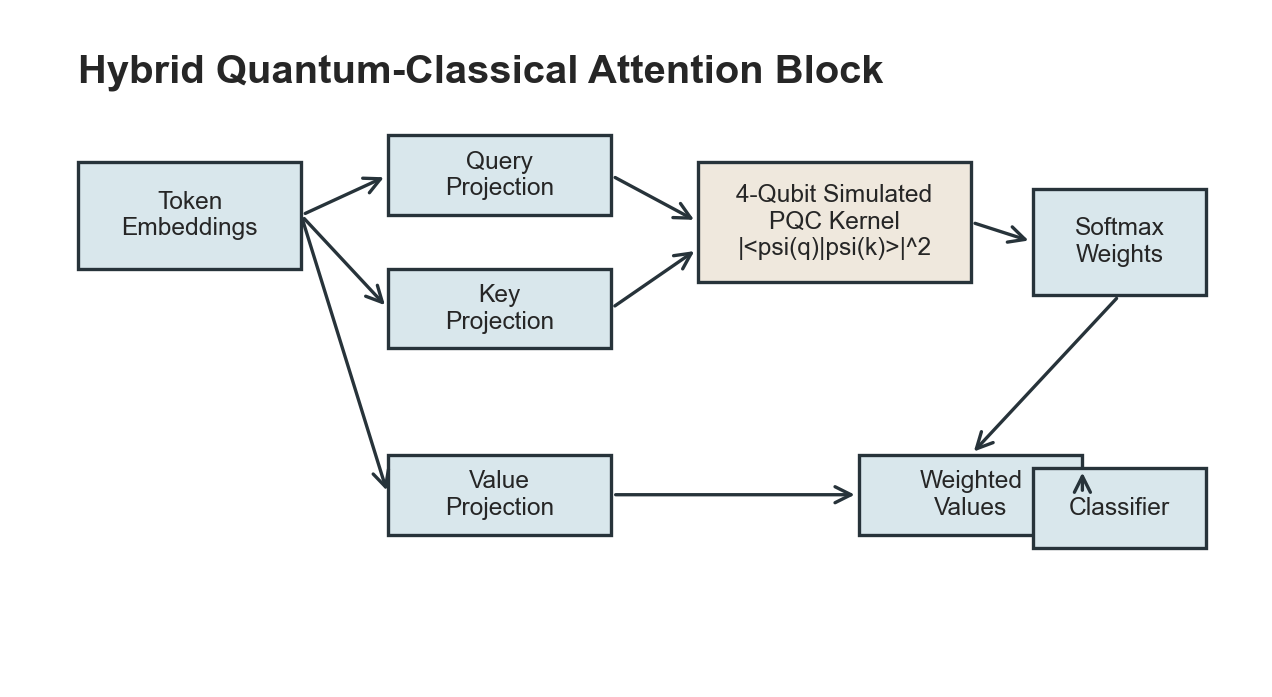
\includegraphics[width=0.95\linewidth]{../figures/architecture_diagram.png}
\caption{Hybrid quantum-classical attention block. Queries and keys are projected into a four-dimensional feature space, encoded into a simulated four-qubit circuit, and compared through quantum-state overlap. Values and the classifier remain classical.}
\label{fig:architecture}
\end{figure}

\subsection{Training and Evaluation}
All models were trained for five epochs with the same dataset split and random seed. Evaluation included test accuracy, macro-F1, loss, runtime scaling, attention-map alignment, gradient variance, and simulated quantum noise. Runtime was measured as mean forward-pass time in milliseconds for sequence lengths 8, 16, 32, and 64 with batch size 32.

Attention-map alignment was measured using linear centered kernel alignment (CKA), a representation-similarity metric used to compare activation or attention structures \cite{kornblith2019similarity}. A low CKA score indicates that two attention maps are structurally different.

\section{Results}
\subsection{Classification Performance}
The classical ablation achieved the strongest test accuracy, followed closely by the standard classical baseline. The hybrid model reached non-trivial performance but trailed both classical models.

\begin{table}[H]
\centering
\caption{Final classification results on the AG News test subset.}
\begin{tabular}{lrrrrr}
\toprule
Model & Accuracy & Macro-F1 & Test Loss & Best Val. Acc. & Train Time (s)\\
\midrule
Classical & 0.769 & 0.768 & 0.734 & 0.752 & 5.65\\
Classical ablation & 0.778 & 0.779 & 0.742 & 0.770 & 5.57\\
Hybrid quantum & 0.706 & 0.705 & 0.815 & 0.723 & 13.84\\
\bottomrule
\end{tabular}
\end{table}

\begin{figure}[H]
\centering
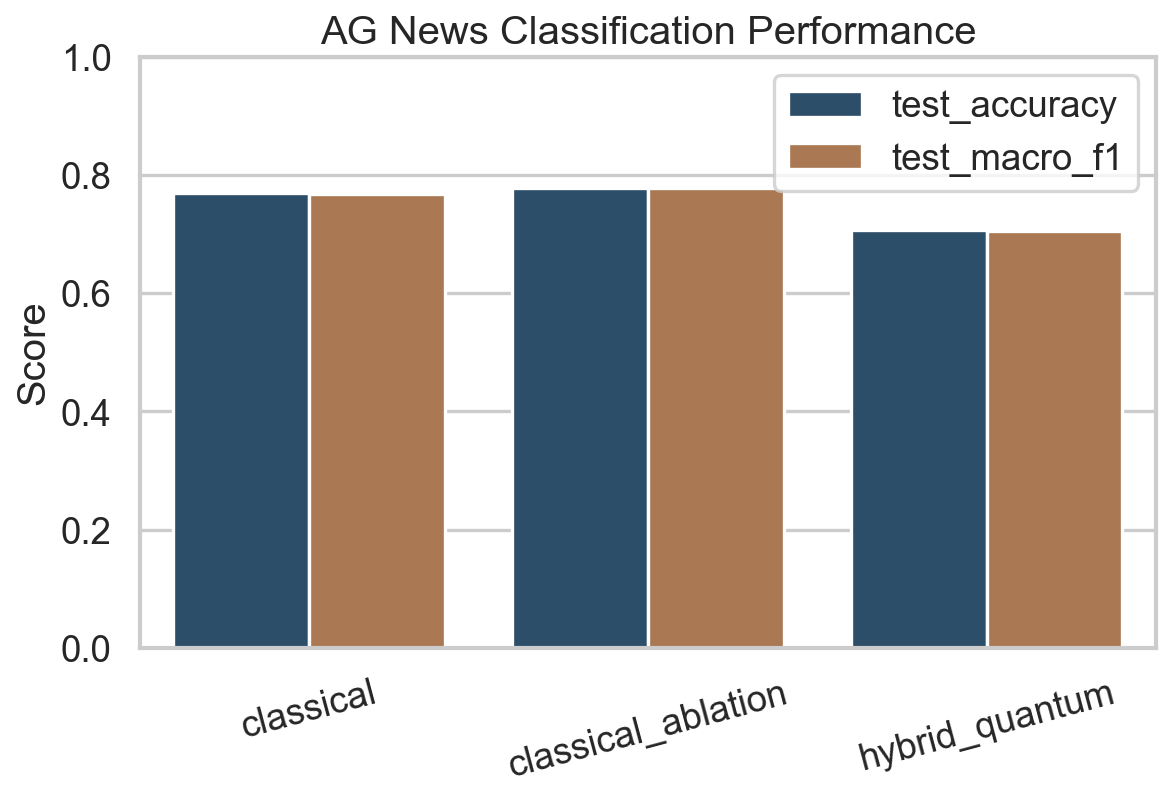
\includegraphics[width=0.82\linewidth]{../figures/accuracy_f1_summary.png}
\caption{Classification accuracy and macro-F1. The low-dimensional classical ablation slightly outperformed the standard classical baseline, while the hybrid quantum model lagged behind both classical alternatives.}
\label{fig:performance}
\end{figure}

\subsection{Runtime Scaling}
The hybrid model was slower at every tested sequence length. At sequence length 32, the hybrid model required 4.16 ms per forward pass, while the classical baseline required 1.39 ms. This makes the hybrid simulation 2.99 times slower at that sequence length.

\begin{table}[H]
\centering
\caption{Mean forward-pass runtime in milliseconds.}
\begin{tabular}{lrrrr}
\toprule
Model & Length 8 & Length 16 & Length 32 & Length 64\\
\midrule
Classical & 0.53 & 0.62 & 1.39 & 2.29\\
Classical ablation & 0.49 & 0.75 & 1.26 & 1.84\\
Hybrid quantum & 1.40 & 3.09 & 4.16 & 6.17\\
\bottomrule
\end{tabular}
\end{table}

\begin{figure}[H]
\centering
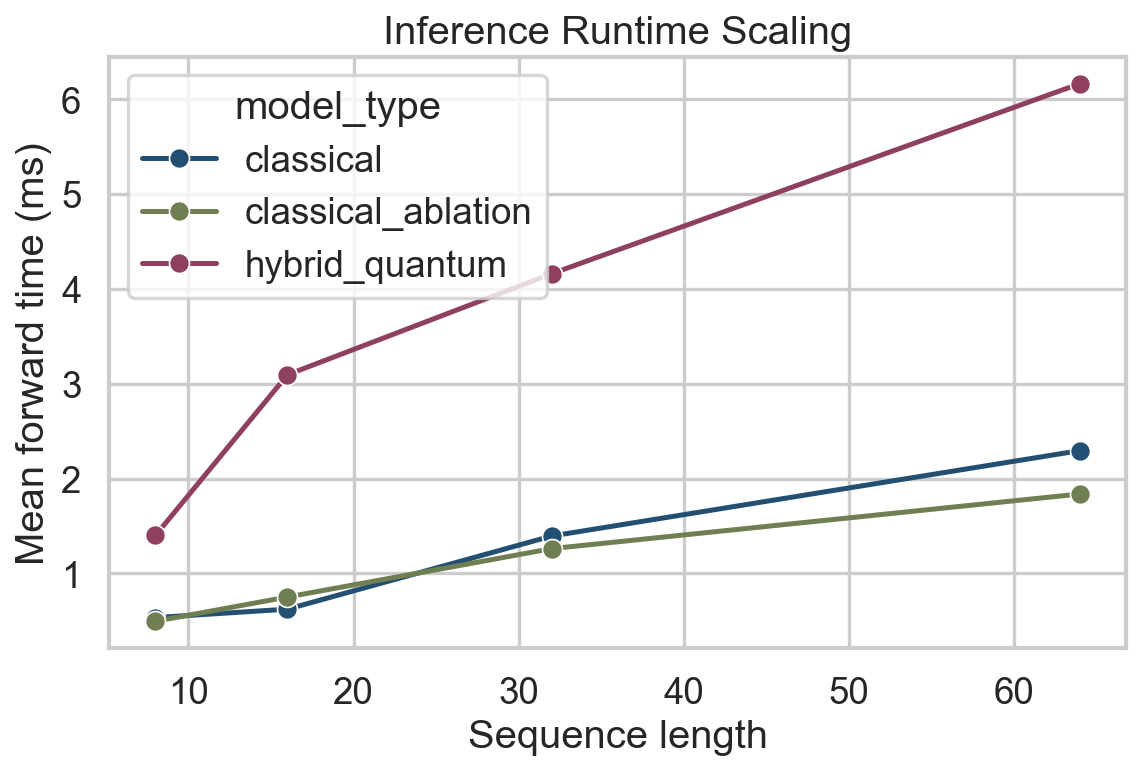
\includegraphics[width=0.82\linewidth]{../figures/benchmark_runtime.png}
\caption{Inference runtime scaling. Under classical state-vector simulation, the hybrid quantum attention block adds overhead rather than reducing empirical runtime.}
\label{fig:runtime}
\end{figure}

\subsection{Attention-Map Alignment}
The hybrid model's attention maps had low CKA alignment with the classical baseline. This suggests that the quantum kernel is not simply reproducing classical dot-product attention; it induces a different similarity structure.

\begin{table}[H]
\centering
\caption{Linear CKA alignment between attention maps.}
\begin{tabular}{lrr}
\toprule
Model Pair & Linear CKA & Mean Absolute Difference\\
\midrule
Classical vs. hybrid quantum & 0.037 & 0.0386\\
Classical vs. classical ablation & 0.100 & 0.0361\\
Classical ablation vs. hybrid quantum & 0.036 & 0.0317\\
\bottomrule
\end{tabular}
\end{table}

\begin{figure}[H]
\centering
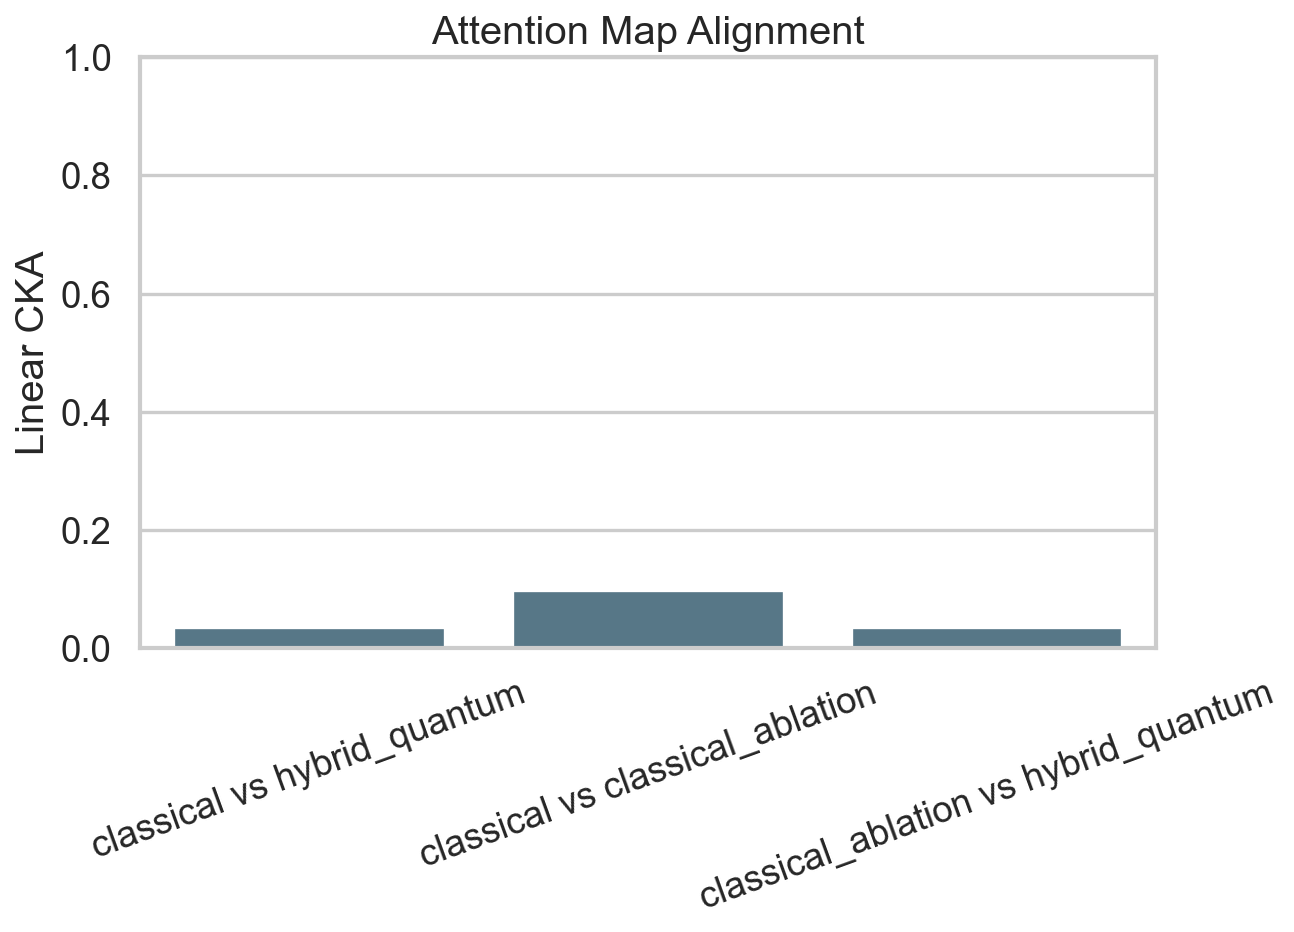
\includegraphics[width=0.82\linewidth]{../figures/attention_alignment.png}
\caption{Attention-map alignment. All alignments are low, but the classical baseline aligns more strongly with the classical ablation than with the hybrid model.}
\label{fig:alignment}
\end{figure}

\subsection{Noise Robustness}
The simulated noise sweep applied angle perturbation and depolarizing-style mixing to the quantum attention component. The hybrid model's accuracy changed from 70.6\% at zero noise to 71.2\% at the highest tested noise level. This small change suggests that the compact model was not highly sensitive to the tested perturbation range, though the result should not be interpreted as hardware-level noise robustness.

\begin{figure}[H]
\centering
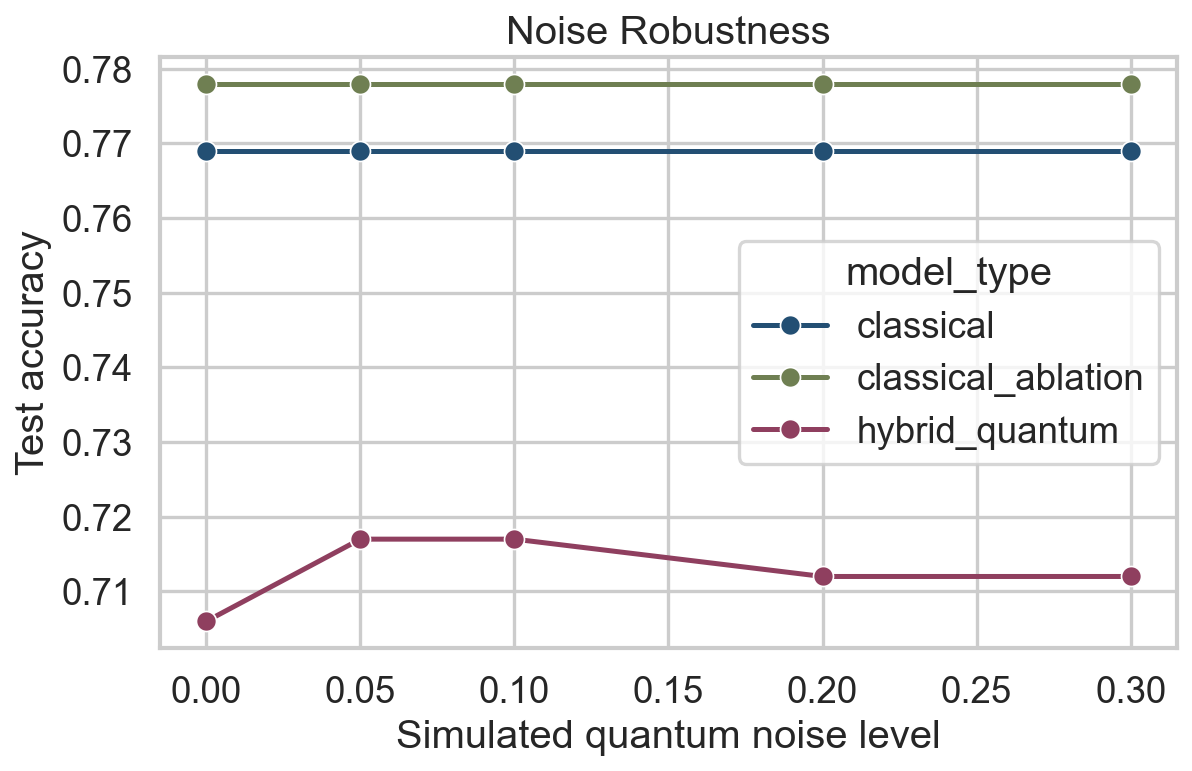
\includegraphics[width=0.82\linewidth]{../figures/noise_robustness.png}
\caption{Noise robustness sweep. Classical models are repeated as references because they do not contain a quantum module. The hybrid model shows only modest accuracy movement under the simulated perturbations.}
\label{fig:noise}
\end{figure}

\subsection{Gradient Variance and Trainability}
Gradient variance changed with circuit depth. It increased from depth 1 to depth 3 and then decreased at depths 4 and 5. This does not show an immediate barren plateau in the tested range, but it does confirm that ansatz depth affects optimization behavior.

\begin{table}[H]
\centering
\caption{Quantum circuit trainability diagnostic.}
\begin{tabular}{rrrr}
\toprule
Circuit Depth & Mean Abs. Gradient & Gradient Variance & Gradient Norm\\
\midrule
1 & 0.00242 & \(1.53\times10^{-5}\) & 0.0114\\
2 & 0.00379 & \(3.56\times10^{-5}\) & 0.0203\\
3 & 0.00387 & \(4.89\times10^{-5}\) & 0.0267\\
4 & 0.00361 & \(4.23\times10^{-5}\) & 0.0283\\
5 & 0.00296 & \(3.48\times10^{-5}\) & 0.0270\\
\bottomrule
\end{tabular}
\end{table}

\begin{figure}[H]
\centering
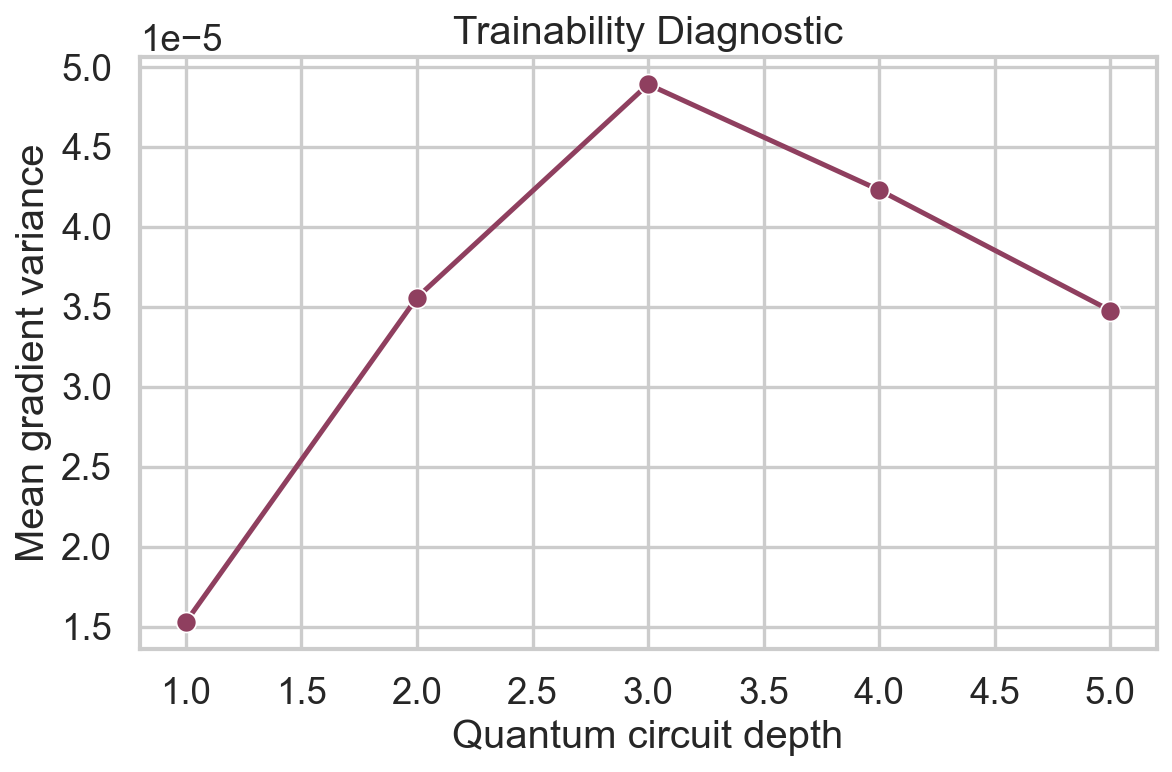
\includegraphics[width=0.82\linewidth]{../figures/gradient_variance.png}
\caption{Trainability diagnostic. Gradient variance peaks at circuit depth 3 and then declines, showing that circuit depth changes optimization behavior even in this compact simulator.}
\label{fig:gradient}
\end{figure}

\section{Discussion}
The experiment supports the feasibility of a hybrid quantum-classical attention block. The model runs end-to-end, trains on a real text dataset, produces attention maps, and can be evaluated with the same metrics as classical baselines. However, the results do not support a near-term practical efficiency advantage under classical simulation. The hybrid model was slower than the classical baseline at every tested sequence length and achieved lower classification accuracy.

The ablation result is especially important. The classical ablation used the same four-dimensional query/key bottleneck as the hybrid model but did not use quantum state overlap. It achieved the highest accuracy in the final run. This implies that dimensionality reduction by itself can be competitive and that the quantum kernel did not provide an advantage on this task. In other words, the observed behavior should not be attributed to quantum geometry unless it exceeds a matched low-dimensional classical control.

At the same time, the low attention-map CKA values show that the hybrid kernel did change the attention structure. The hybrid model did not merely mimic classical dot-product attention. That difference may be useful in future settings, but in this experiment the different geometry did not translate into better accuracy or runtime. This distinction is scientifically valuable because it separates novelty from advantage.

\section{Limitations}
Several limitations shape the interpretation of this project. First, the quantum circuit is simulated on classical hardware. The measured runtime therefore reflects state-vector simulation overhead, not the speed of a real quantum processor. Second, the experiment uses a small classifier rather than a large language model. This is appropriate for a reproducible senior research project, but it means the conclusions should not be generalized to production-scale LLMs. Third, the AG News dataset is a short-text classification benchmark, not a long-context generation task. Finally, the circuit uses only four qubits and a simple hardware-efficient ansatz. Other encodings, circuit structures, or noise models could produce different results.

\section{Conclusion}
This project implemented a reproducible hybrid quantum-classical attention mechanism that isolates the query-key similarity computation inside an otherwise classical attention block. The hybrid model successfully trained and produced measurable attention behavior, demonstrating feasibility. However, it did not outperform the classical baselines and was approximately 2.99 times slower than classical attention at sequence length 32 under state-vector simulation. The strongest contribution is therefore methodological: the project provides a controlled framework for comparing quantum kernels, classical attention, and matched ablation models using accuracy, runtime, alignment, gradient variance, and noise robustness.

\section{Future Work}
Future work should test the hybrid attention block on longer sequences, larger datasets, and alternative circuit ansatzes. More realistic quantum-noise simulations would help determine whether the observed noise stability persists under hardware-like conditions. The most important next step is to evaluate whether actual quantum hardware can compute the kernel more efficiently than classical state-vector simulation. Until then, claims about quantum attention should be framed carefully: feasibility is demonstrated here, but practical advantage is not.

\appendix
\section{Reproducibility Notes}
The codebase contains a full project pipeline. The main experiment can be run with:
\begin{verbatim}
.venv/bin/python scripts/run_all.py --train-size 5000 --val-size 1000 \
  --test-size 1000 --epochs 5 --benchmark-repeats 8
\end{verbatim}
The output metrics are stored in \texttt{results/metrics/}, figures in \texttt{figures/}, and final artifacts in \texttt{paper/} and \texttt{poster/}. The repository excludes the virtual environment, cache folders, training checkpoints, and temporary QA renderings.

\section{Generated Project Figures}
\begin{figure}[H]
\centering
\begin{subfigure}{0.48\linewidth}
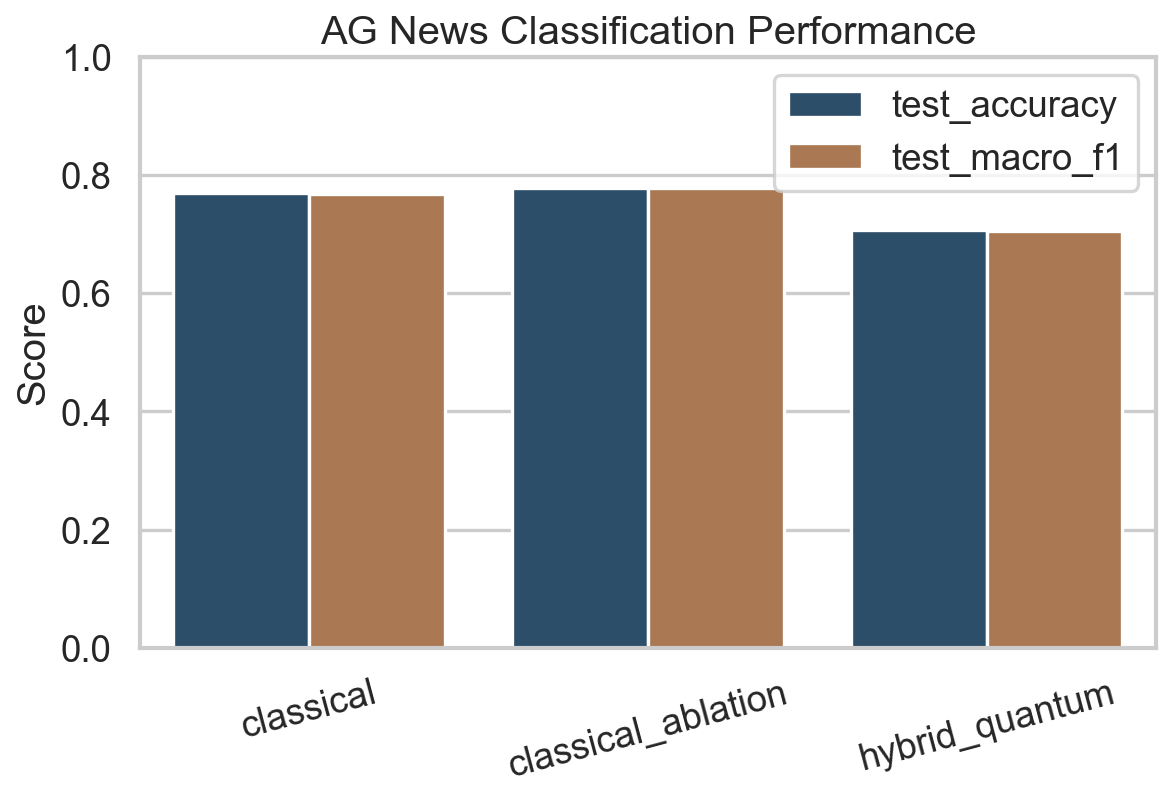
\includegraphics[width=\linewidth]{../figures/accuracy_f1_summary.png}
\caption{Classification scores.}
\end{subfigure}
\begin{subfigure}{0.48\linewidth}
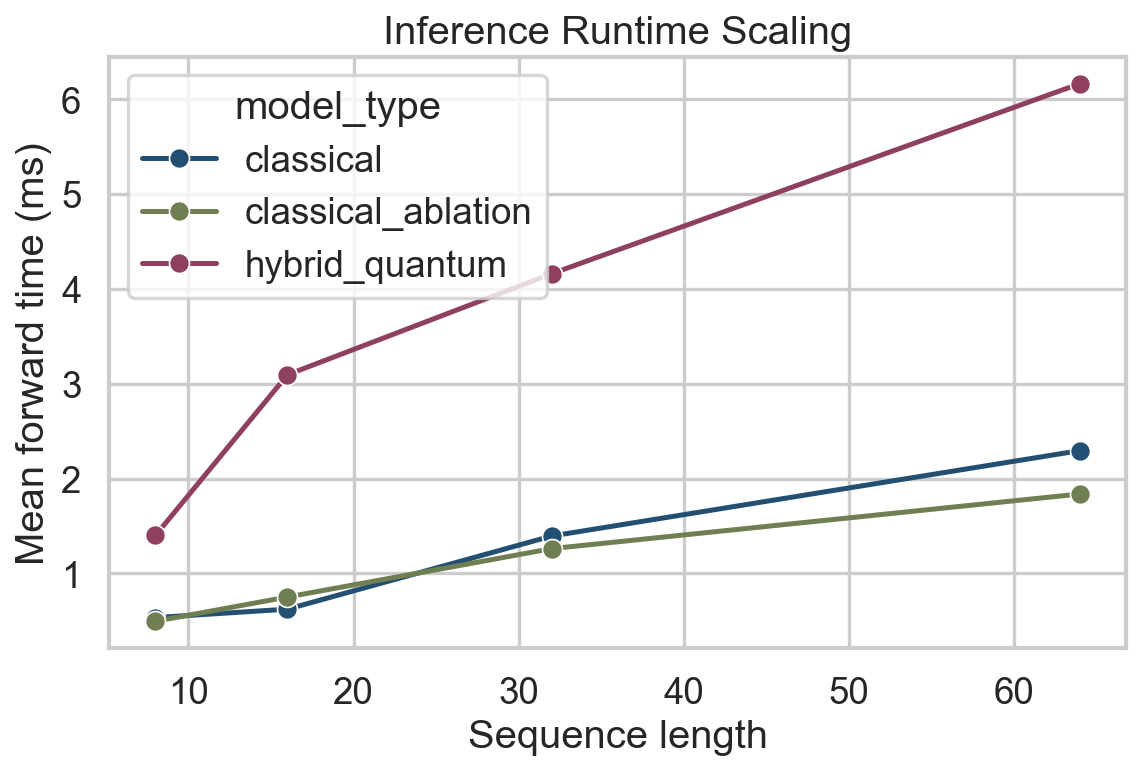
\includegraphics[width=\linewidth]{../figures/benchmark_runtime.png}
\caption{Runtime scaling.}
\end{subfigure}
\begin{subfigure}{0.48\linewidth}
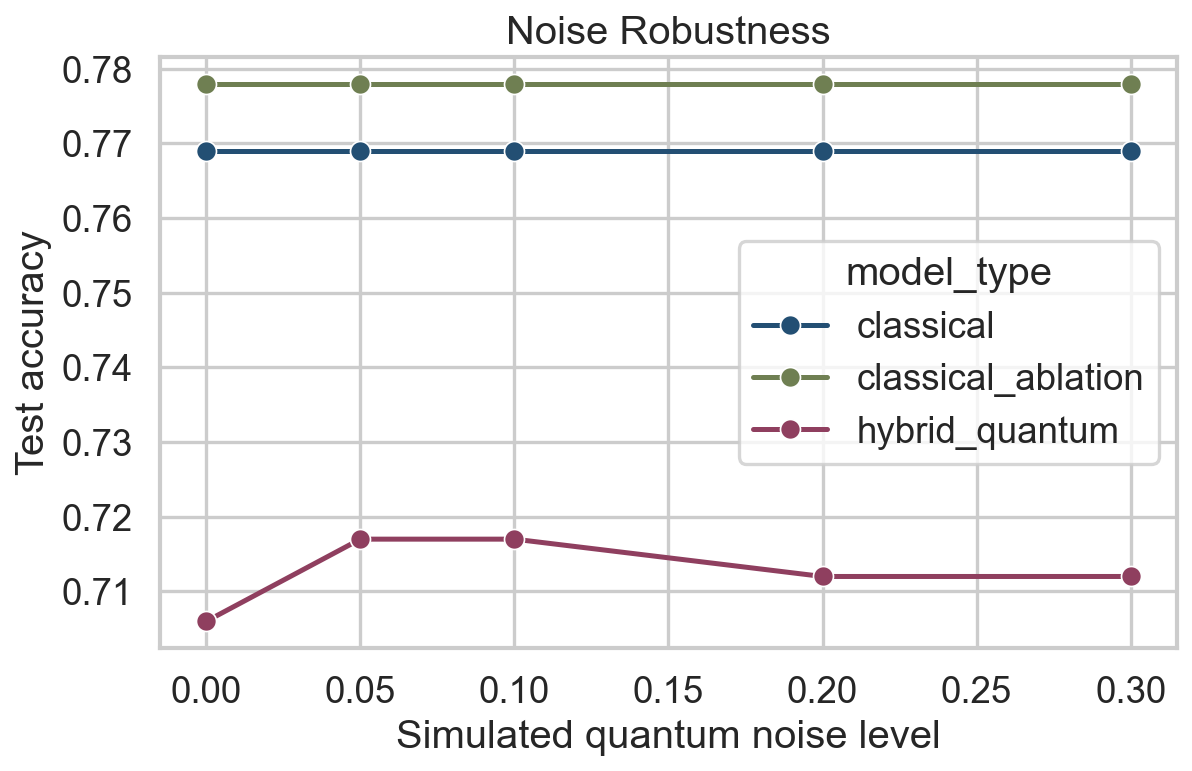
\includegraphics[width=\linewidth]{../figures/noise_robustness.png}
\caption{Noise sweep.}
\end{subfigure}
\begin{subfigure}{0.48\linewidth}
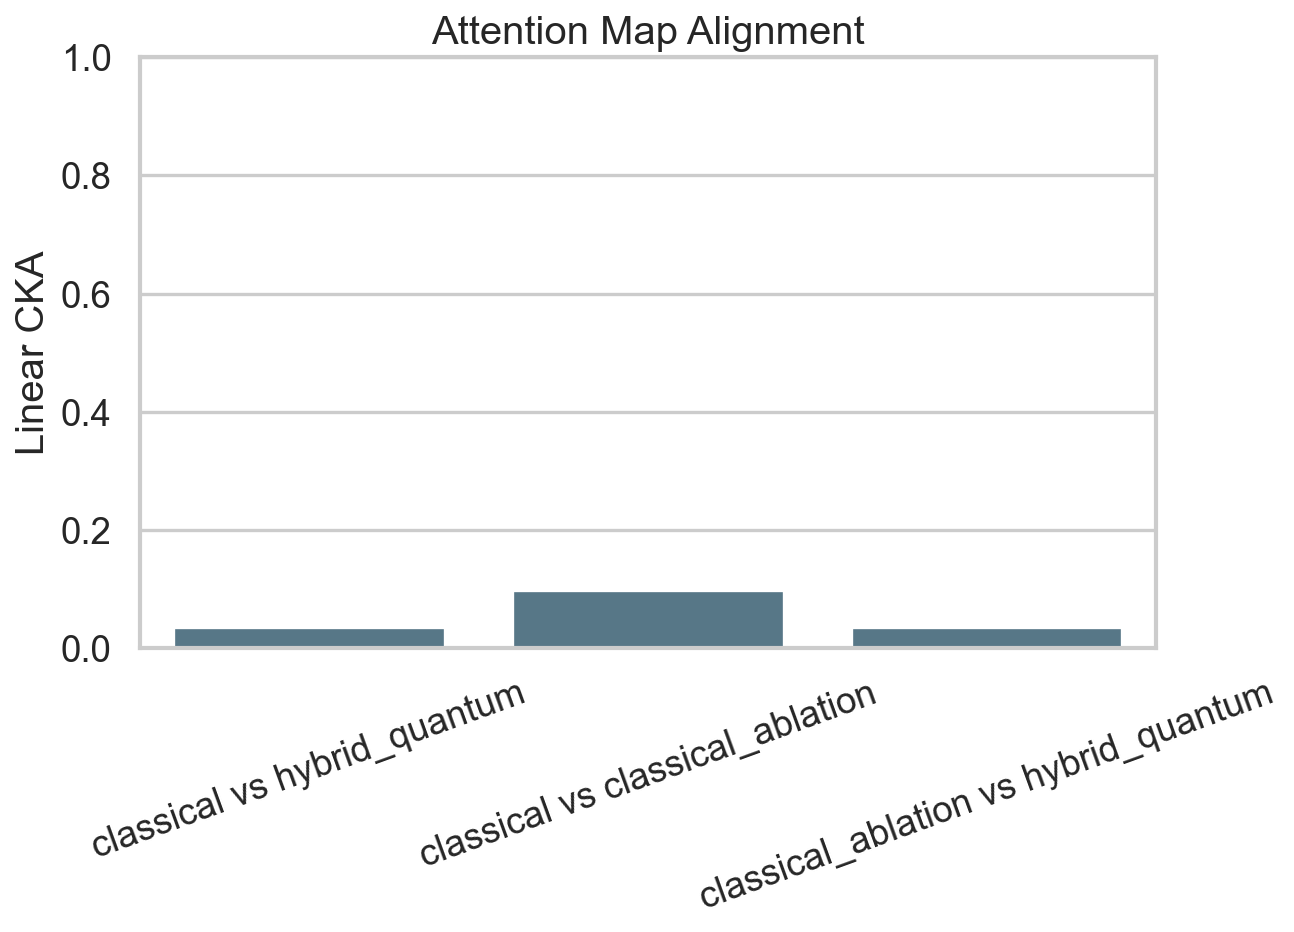
\includegraphics[width=\linewidth]{../figures/attention_alignment.png}
\caption{Attention alignment.}
\end{subfigure}
\caption{Summary of generated project figures used in the poster and report.}
\end{figure}

\bibliographystyle{plain}
\bibliography{references}

\end{document}

